\begin{figure*}[h]
  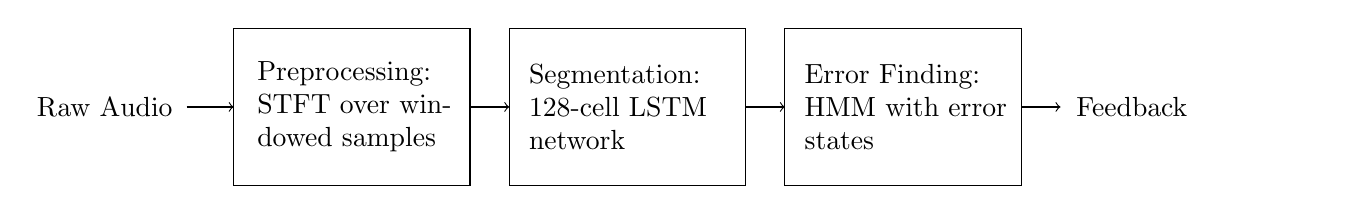
\begin{tikzpicture}
    \centering
    % raw audio
    \node[text width=3cm] at (-1, 1) {Raw Audio}; 
    \draw [->] (-0.6, 1) -- (0, 1);
    % preprocessing
    \draw (0, 0) -- (3, 0) -- (3, 2) -- (0, 2) -- cycle;
    \node[text width=3.2cm] at (1.9, 1) {Preprocessing: \\ STFT over windowed samples};
    \draw [->] (3, 1) -- (3.5, 1);
    % segmentation
    \draw (3.5, 0) -- (6.5, 0) -- (6.5, 2) -- (3.5, 2) -- cycle;
    \node[text width=2.7cm] at (5.1, 1) {Segmentation: \\ 128-cell LSTM network};
    \draw [->] (6.5, 1) -- (7, 1);
    % error finding
    \draw (7, 0) -- (10, 0) -- (10, 2) -- (7, 2) -- cycle;
    \node[text width=2.7cm] at (8.6, 1) {Error Finding: \\ HMM with error states};
    \draw [->] (10, 1) -- (10.5, 1);
    % feedback
    \node[text width=3cm] at (12.2, 1) {Feedback};
  \end{tikzpicture}
  \centering
  \caption{The overall architecture of our piano tutor. The specifics, such as the size and depth of the neural network and the exact preprocessing steps, apply only to the piano tutor. However, the overall architecture can theoretically be extended to pronunciation tutoring and other tutoring problem domains.}
  \label{fig:arch}
\end{figure*}